% БҮЛЭГ 4 — ӨГӨГДЛИЙН БОЛОВСРУУЛАЛТ
% Эх: diploma_0.2v.docx, БҮЛЭГ 4. ӨГӨГДЛИЙН БЭЛТГЭЛ

\chapter{Өгөгдлийн боловсруулалт}
\label{Chapter4}

%-------------------------------------------------------------------------------
\section{Өгөгдлийн цуглуулалт}

Системийн сургалтын болон туршилтын өгөгдлийн багц нь нийт \textbf{найман}
нийтэд нээлттэй эх сурвалжаас бүрдэнэ (задаргааг Хүснэгт~\ref{tab:data_full_corpus}):
news.mn (42.3\%), gogo.mn (28.1\%), IKON.mn (9.2\%), E-Mongolia (6.4\%),
Facebook-ийн ``Мэдэхгүй зүйлээ асуу'' групп (6.3\%), Medee.mn (3.4\%),
Zaluusinfo (2.3\%), Eagle News (1.9\%). Дийлэнх хувь ($\approx$91\%) нь мэдээний
сайтуудын нийтийн сэтгэгдлийн хэсгээс, харин $\approx$6.3\% нь Facebook-ийн нээлттэй
группээс бүрдэнэ. Олон эх сурвалжаас цуглуулсан үндэслэл нь домайны олон талт
байдлыг (domain diversity) хангах явдал юм --- зөвхөн нэг платформоос авсан
өгөгдөл загварыг тухайн платформын хэлбэр, ярианы хэв маягт хэт тохируулж болзошгүй.

\textbf{Кирилл бичгийн шүүлтийн шалгуур.} Цуглуулалтын шатанд кирилл
тэмдэгтийн эзлэх хувийг тооцоолох автомат шүүлтийн алхам хэрэгжүүлнэ. Нийт
тэмдэгтийн $85$ хувиас дээш нь кирилл тэмдэгт байхыг шаардлага болгох бөгөөд
энэ босгоос доогуур текстийг датасетад оруулахгүй. Латин үсгийн бичвэр,
монгол-англи холимог (code-switched) текст, болон латин үсгийн хэлбэртэй Монгол бичлэг
(жишээлбэл ``bn'', ``yu ve'', ``zgr'') бүгд хасагдана. Энэхүү шийдэл нь
MN-BERT-ийн кирилл корпус дээр суурилсан токенчлолын үр ашгийг бүрэн
хэрэгжүүлэхэд зайлшгүй шаардлагатай.

Мэдээний сайтуудын (news.mn, gogo.mn, IKON.mn гэх мэт) сэтгэгдлүүд нь нийгэм,
улс төр, эдийн засаг, спорт, соёл зэрэг олон сэдвийг хамарсан, харьцангуй урт,
бичгийн хэлний шинжтэй байдаг. Харин Facebook-ийн нээлттэй группийн сэтгэгдэлд
ярианы хэлний хэлбэр, emoji агуулсан богино сэтгэгдлүүд зонхилдог тул
хэрэглэгчдийн бодит онлайн харилцааны хэв маягийг илүү сайн тусгаж өгдөг.
Энэ хэсгээс цуглуулсан өгөгдөлд кирилл бичгийн шүүлтийн алхам онцгой чухал
байдаг бөгөөд учир нь латин үсгийн бичлэг болон code-switching харьцангуй
түгээмэл тохиолддог. Ийнхүү шинж чанараараа ялгаатай олон эх сурвалжаас
цуглуулсан, кирилл шүүлтийг давсан өгөгдлийн багц нь загварын хэрэглэгдэх
орчны олон талт байдлыг хангах боломжийг бүрдүүлнэ.

Цуглуулалтын техникийн хувьд: news.mn-ийн хувьд сайтын ачааллыг тооцоолсон
web scraping ашиглана; Facebook-ийн хувьд Graph API-ийн нийтийн мэдээллийн
хандалтын боломжид тулгуурлана. Цуглуулах хугацааны хүрээ нь 2025--2026 оны эхэн
байх бөгөөд домайны тэнцвэргүй байдлыг (domain bias) бууруулахын тулд сэдэв
болон платформ бүрээс жигд хувь авах stratified sampling арга ашиглана.

Шошголсон 10,000 дээжийн ангиллын бүтцийг Хүснэгт~\ref{tab:collection}-д,
эх сурвалжийн тархалтыг Хүснэгт~\ref{tab:data_full_corpus}-д нэгтгэсэн бол
харааны шинжилгээг Зураг~\ref{fig:data_analysis_combined}-д харуулав.

\begin{table}[H]
\centering
\caption{Ангилал тус бүрийн шошгологдсон сэтгэгдлийн тоо (n=10{,}000;
  эх сурвалжийн задаргааг Хүснэгт~\ref{tab:data_full_corpus}-аас үзнэ үү)}
\label{tab:collection}
\begin{tabular}{@{}lcc@{}}
\toprule
\textbf{Ангилал} & \textbf{Нийт сэтгэгдэл} & \textbf{Хувь (\%)} \\
\midrule
Бүтээлч шүүмжлэл  & $4{,}356$ & $43.56\%$ \\
Саармаг           & $3{,}026$ & $30.26\%$ \\
Хортой сөрөг      & $1{,}963$ & $19.63\%$ \\
Эерэг             & $655$     & $6.55\%$  \\
\midrule
\textbf{Нийт}   & $\mathbf{10{,}000}$ & $\mathbf{100\%}$ \\
\bottomrule
\end{tabular}
\end{table}

% ── Шошголсон өгөгдлийн эх сурвалжийн хүснэгт (10k) ────────────────────────
\begin{table}[H]
\centering
\caption{Шошголсон өгөгдлийн эх сурвалжийн тархалт (n=10{,}000)}
\label{tab:data_full_corpus}
\begin{tabular}{@{}lcc@{}}
\toprule
\textbf{Эх сурвалж} & \textbf{Тоо} & \textbf{Хувь (\%)} \\
\midrule
news.mn                & $4{,}230$ & $42.3\%$ \\
gogo.mn                & $2{,}811$ & $28.1\%$ \\
IKON.mn                & $919$     & $9.2\%$  \\
E-Mongolia             & $644$     & $6.4\%$  \\
Мэдэхгүй зүйлээ асуу  & $632$     & $6.3\%$  \\
Medee.mn               & $342$     & $3.4\%$  \\
Zaluusinfo             & $234$     & $2.3\%$  \\
Eagle News             & $188$     & $1.9\%$  \\
\midrule
\textbf{Нийт} & $\mathbf{10{,}000}$ & $\mathbf{100\%}$ \\
\bottomrule
\end{tabular}
\end{table}

Эх сурвалж тус бүрийн ангиллын задаргааг (аль өгөгдөл аль ангилалд хамаарсан)
Хүснэгт~\ref{tab:source-category}-д үзүүлэв.

\begin{table}[H]
\centering
\caption{Эх сурвалж $\times$ ангиллын задаргаа (n=10{,}000)}
\label{tab:source-category}
\fittable{%
\begin{tabular}{@{}lccccc@{}}
\toprule
\textbf{Эх сурвалж} & \textbf{Бүтээлч} & \textbf{Саармаг} & \textbf{Эерэг} & \textbf{Хортой} & \textbf{Нийт} \\
\midrule
news.mn               & $2{,}050$ & $920$ & $239$ & $1{,}021$ & $4{,}230$ \\
gogo.mn               & $1{,}417$ & $623$ & $191$ & $580$ & $2{,}811$ \\
IKON.mn               & $313$ & $371$ & $59$ & $176$ & $919$ \\
E-Mongolia            & $296$ & $315$ & $33$ & $0$ & $644$ \\
Мэдэхгүй зүйлээ асуу & $37$ & $523$ & $40$ & $32$ & $632$ \\
Medee.mn              & $123$ & $112$ & $29$ & $78$ & $342$ \\
Zaluusinfo            & $35$ & $106$ & $54$ & $39$ & $234$ \\
Eagle News            & $85$ & $56$ & $10$ & $37$ & $188$ \\
\midrule
\textbf{Нийт} & $\mathbf{4{,}356}$ & $\mathbf{3{,}026}$ & $\mathbf{655}$ & $\mathbf{1{,}963}$ & $\mathbf{10{,}000}$ \\
\bottomrule
\end{tabular}}
\end{table}

% ── Харааны шинжилгээний зураг ───────────────────────────────────────────────
\begin{figure}[H]
  \centering
  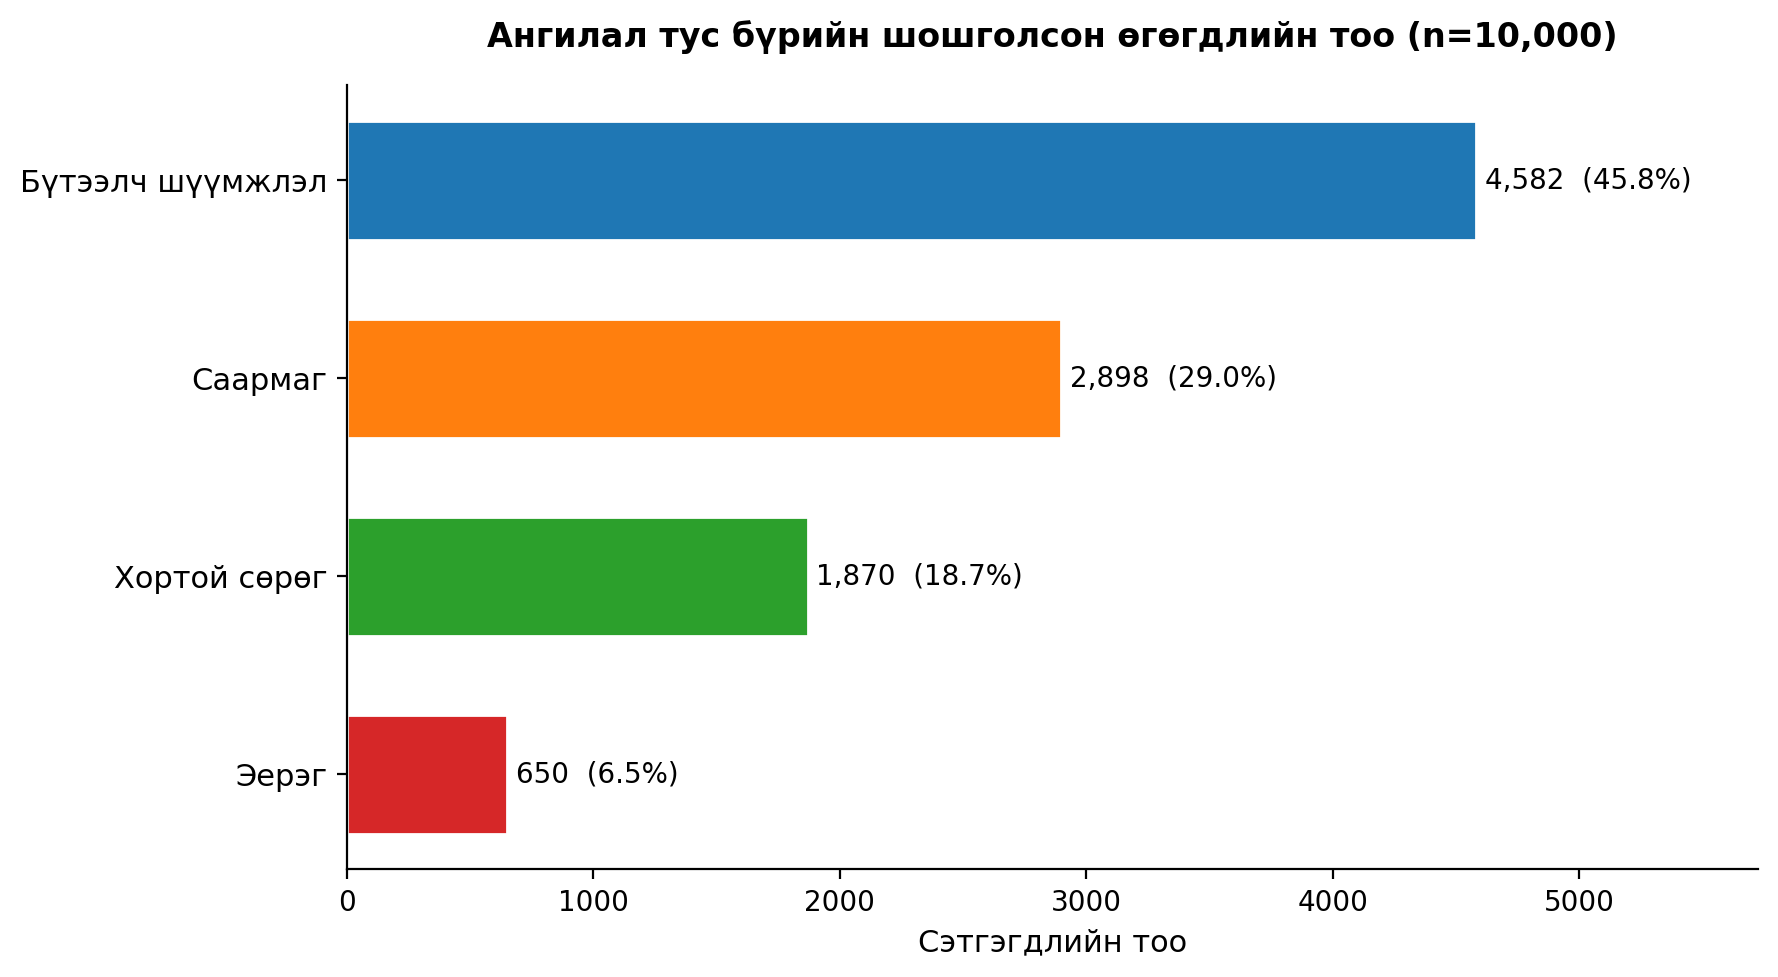
\includegraphics[width=0.78\textwidth]{Figures/data_categories_bar.png}
  \caption{Шошголсон 10,000 дээжийн ангиллын тархалт. Бүтээлч шүүмжлэл ангилал
    (43.56\%) тодорхой давамгайлж байна.}
  \label{fig:data_analysis_combined}
\end{figure}

Шошголсон өгөгдлийн ангиллын тархалтаас харахад (Хүснэгт~\ref{tab:collection};
Зураг~\ref{fig:data_analysis_combined}) Бүтээлч шүүмжлэл ангилал (43.56\%) давамгайлж,
Эерэг ангилал (6.55\%) хамгийн цөөн дээжтэй байна. Өөрөөр хэлбэл, хамгийн их
ба хамгийн бага ангиллын дээжийн тоо ойролцоогоор $6.6{:}1$ харьцаатай буюу тэнцвэргүй
байдал тодорхой илэрч байна. Энэ тэнцвэргүй байдлыг шийдвэрлэхдээ суурь загваруудад
(LR, NB, SVM) SMOTE, эцсийн нэг шатлалт MN-BERT загварт ангиллын жин оногдуулсан
Focal Loss ($\gamma=2.0$) болон WeightedRandomSampler-ийг хослуулан хэрэглэсэн
(бүлэг~\ref{Chapter5}).

%-------------------------------------------------------------------------------
\section{Өгөгдлийн цэвэрлэгээ ба урьдчилсан боловсруулалт}

Цуглуулсан хам текст (raw text) нь олон хэлбэрийн дуу чимээ (noise) агуулдаг
тул системчилсэн цэвэрлэгээний pipeline (урьдчилсан боловсруулалтын дамжлага) зайлшгүй
шаардлагатай. Боловсруулалтын дараах үе шатуудыг дараалсан байдлаар хэрэгжүүлнэ.

\textbf{Кирилл хүчинтэй байдлын шүүлт (Cyrillic validation filtering).}
Pipeline-ийн эхний алхам болгон кирилл хүчинтэй байдлын шүүлт хэрэгжүүлнэ.
Тус алхам нь Unicode тэмдэгтийн ангиллыг ашиглан кирилл тэмдэгтийн харьцааг
тооцоолно. Кирилл тэмдэгтийн эзлэх хувь нийт утгатай тэмдэгтийн 85 хувиас
доогуур байвал тухайн бичвэрийг хасна (бүлэг~\ref{Chapter4}-ийн эхэнд заасан
$\geq 85\%$ кирилл шаардлагатай нийцнэ). Уг босго нь тоо, цэг таслал зэрэг кирилл бус боловч утгатай
тэмдэгтүүдийг зөвшөөрч, цэвэр латин болон code-switched текстийг хасахаар
тохируулагдана. Энэхүү алхам нь токенчлол болон бусад боловсруулалтын алхамуудын
өмнө явагдах нь чухал, учир нь MN-BERT-ийн vocabulary нь кирилл корпус дээр
суурилсан тул кирилл бус текст токенчлолын чанарыг эрс бууруулна.

\textbf{Текст нормчлол.} HTML тэмдэгт болон URL хаягийг хасна; тусгай тэмдэгт
болон тоог тохирсон нэрлэсэн токенд (placeholder token) хөрвүүлнэ. Emoji-г preprocessing явцад устгахын оронд \texttt{[EMOJI]} гэсэн placeholder
токен болгон хөрвүүлнэ. Энэ нь өгүүлбэрийн токений байрлалыг хадгалж,
MN-BERT токенчлолын тогтвортой байдлыг хамгаалах зорилготой. Гэхдээ
\texttt{[EMOJI]} токен нь загварын утга-семантик боловсруулалтад хувь нэмэр
оруулахгүй --- зөвхөн байрлалын тэмдэглэгчийн үүрэг гүйцэтгэнэ. Давтагдсан цагаан зай болон шугам завсар зэргийг
мөн арилгана.

\textbf{Токенчлол.} Монгол хэлний agglutinative онцлогт тохируулсан MN-BERT-ийн
SentencePiece tokenizer ашиглана. Энэ tokenizer нь Монгол кирилл корпус дээр
сургагдсан тул кирилл бичгийн нийлмэл нөхцөлт үгийн бүтцийг морфологийн
тогтвортой байдлаар дэд үгийн (subword) түвшинд задалдаг. Кирилл шүүлтийг давсан
өгөгдөл дээр тус tokenizer оновчтой ажиллах тул дээрх шүүлтийн алхам болон энэ
алхам хоорондоо нягт уялдаатай.

\textbf{Зөвхөн суурь загварт: стоп үг хасах ба stemming.} Стоп үг хасах
(``нь'', ``бол'', ``байна'', ``гэж'' гэх мэт) болон үгийн үндэс олох (stemming)
алхмууд нь \emph{зөвхөн TF-IDF суурьтай суурь загваруудад} (LR, NB, SVM)
хамаарна --- учир нь эдгээр статистик арга нь морфологийн хувьслыг өөрөө
боловсруулж чаддаггүй. \textbf{MN-BERT загвар эдгээр алхмыг ашигладаггүй:}
BERT нь дэд үгийн (subword) SentencePiece токенчлолоор agglutinative
морфологийг дотооддоо боловсруулдаг тул нормчлогдсон текстийг шууд хүлээн авна.
Иймд MN-BERT-ийн боловсруулалтын дараалал нь: кирилл шүүлт $\to$ текст нормчлол
$\to$ SentencePiece токенчлол (стоп үг хасах, stemming \emph{хийхгүй}).

%-------------------------------------------------------------------------------
\section{Шошгологдолтын стратеги}

Өгөгдлийн шошгололт нь дөрвөн ангилалыг хамарна: \textbf{Эерэг} (эерэг хандлага,
сайшаал), \textbf{Саармаг} (мэдээллийн, саармаг тайлбар), \textbf{Хортой сөрөг}
(хувь хүнд чиглэсэн доромжлол, дарамт, заналхийлэл),
\textbf{Бүтээлч шүүмжлэл} (аргументтай, шийдэл санал агуулсан сөрөг хандлага).
Монгол хэлийг эх хэл болгон ярьдаг, Монголын цахим орчны хэлэлцүүлэгтэй танил нийт 3 шошгологч тус дөрвөн ангилалд тохирсон нарийн, тодорхой зааврын дагуу
ажилласан.

Шошгологдолтыг дараах 3 алхамаар зохион байгуулсан:

\begin{enumerate}
  \item \textbf{Зааврын боловсруулалт.} Ангилал тус бүрийн тодорхойлолт, хилийн
    тохиолдлын жишээ, ирони таних зарчим бүхий бичгийн удирдамж бэлтгэв.
  \item \textbf{Бие даасан шошгологдолт.} 3 шошгологч бие биенээсээ хамааралгүй
    бүх 10,000 дээжийг шошголов. Объектив хил хязгаарыг хадгалахын тулд
    ангилалын тодорхойлолтыг зааврын дагуу нарийн мөрдөв.
  \item \textbf{Нийцлийн хэмжилт ба зөрөлдөөн шийдвэрлэлт.} Fleiss' $\kappa$
    коэффициентээр нийцлийг тооцоолж, зөрөлдсөн тохиолдлуудыг 3 шошгологчийн
    хэлэлцэлтээр шийдэв.
\end{enumerate}

\textbf{Кирилл-онцлогт аннотацийн заавар.} Аннотаторуудад зориулсан гарын авлага
дараах тусгай зааврыг агуулна. Нэгдүгээрт, аннотацид оруулах зөвхөн кирилл
бичгийн текстийг л авч үзнэ --- латин тэмдэгт давамгайлсан, code-switched, эсвэл
латин үсгийн хэлбэртэй бичлэг бүхий жишээ аннотацид оруулахгүй бөгөөд эдгээр нь
preprocessing шатанд аль хэдийн хасагдсан байна. Хоёрдугаарт, кирилл бичиглэлтэй
ч агуулгын утга нь тодорхойгүй бол тухайн жишээг ``дүйцэшгүй'' (ambiguous)
хэмээн тэмдэглэж annotation-оос хасна. Гуравдугаарт, Монгол хэлний ирони болон
нутгийн хэлний кирилл хэллэгийг зөв тайлбарлах тусгай жишээ тохиолдлуудыг
гарын авлагад оруулна --- тухайлбал, ``муу'' гэсэн үг сайшаалыг илэрхийлж болох
тул контекстийн дагуу шошгологдолт хийх шаардлага байна.

Шошгологчдын хоорондын нийцлийг хэмжихэд Fleiss' Kappa коэффициент ашиглана.
$\kappa = 0.72$ утга гарсан нь хангалттай нийцлийг илтгэх бөгөөд зөрөлдсөн тохиолдлуудыг
хэлэлцэж, консенсусын дүгнэлт гаргасан.
Аннотацийн бүхий л үйл явцыг зураг~\ref{fig:annotation-process}-д харуулав.

\begin{figure}[H]
\centering
\begin{tikzpicture}[
  mainbox/.style={draw, rounded corners=5pt, minimum width=5.5cm,
                  minimum height=1.20cm, text width=5.1cm,
                  align=center, font=\small, line width=0.8pt},
  annotbox/.style={draw, rounded corners=5pt, minimum width=2.8cm,
                   minimum height=1.20cm, text width=2.5cm,
                   align=center, font=\small, line width=0.8pt},
  decbox/.style={diamond, draw, aspect=2.8, minimum width=3.8cm,
                 inner sep=2pt, align=center, font=\small, line width=0.8pt},
  arr/.style={->, >=Stealth, thick, line width=0.9pt},
]

% ── INPUT ────────────────────────────────────────────────────────────────
\node[mainbox, fill=gray!12, draw=gray!50] (inp) at (0, 0)
  {\textbf{Хам сэтгэгдэл}\\[1pt]
   {\scriptsize $n = 10{,}000$ · найман эх сурвалж}};

% ── ANNOTATION GUIDELINES ────────────────────────────────────────────────
% gap: 2.20 - 0.60 - 0.60 = 1.00 cm
\node[mainbox, fill=blue!10, draw=blue!45] (guide) at (0,-2.20)
  {\textbf{Аннотацийн заавар}\\[1pt]
   {\scriptsize Хил хязгаар · ирони · дүйцэшгүй тохиолдол}};

% ── 3 ANNOTATORS (side by side) ──────────────────────────────────────────
% vertical gap from guide.south(-2.80) to a2.north(-3.80) = 1.00 cm
\node[annotbox, fill=orange!14, draw=orange!55] (a1) at (-3.5,-4.40)
  {\textbf{Шошгологч 1}\\[1pt]
   {\scriptsize Бие даан\\шошголоно}};
\node[annotbox, fill=orange!14, draw=orange!55] (a2) at (0,-4.40)
  {\textbf{Шошгологч 2}\\[1pt]
   {\scriptsize Бие даан\\шошголоно}};
\node[annotbox, fill=orange!14, draw=orange!55] (a3) at (3.5,-4.40)
  {\textbf{Шошгологч 3}\\[1pt]
   {\scriptsize Бие даан\\шошголоно}};

% ── KAPPA MEASUREMENT ────────────────────────────────────────────────────
% gap: 6.60 - 4.40 - 0.60 - 0.60 = 1.00 cm
\node[mainbox, fill=yellow!18, draw=yellow!70!black] (kappa) at (0,-6.60)
  {\textbf{Нийцлийн хэмжилт}\\[1pt]
   {\scriptsize Fleiss' $\kappa = 0.72$ · хангалттай нийцэл}};

% ── DISAGREEMENT DECISION ────────────────────────────────────────────────
% kappa.south=-7.20; dec.north=-8.22 → gap=1.02 cm
\node[decbox, fill=yellow!20, draw=yellow!70!black] (dec) at (0,-8.90)
  {Зөрөлдөөн?};

% ── CONSENSUS (right of diamond) ─────────────────────────────────────────
% dec.east=1.90; cons.west=5.80-2.75=3.05 → gap=1.15 cm
\node[mainbox, fill=red!8, draw=red!40] (cons) at (5.80,-8.90)
  {\textbf{Консенсус хэлэлцэх}\\[1pt]
   {\scriptsize Зөрөлдсөн дээжийг\\3 шошгологч ярилцана}};

% ── FINAL LABEL ──────────────────────────────────────────────────────────
% dec.south=-9.58; final.north=-10.53 → gap=0.95 cm
\node[mainbox, fill=green!14, draw=green!55] (final) at (0,-11.13)
  {\textbf{Эцсийн шошго}\\[1pt]
   {\scriptsize Эерэг · Саармаг · Хортой сөрөг · Бүтээлч шүүмжлэл}};

% ── OUTPUT DATASET ───────────────────────────────────────────────────────
% gap: 13.33 - 11.13 - 0.60 - 0.60 = 1.00 cm
\node[mainbox, fill=blue!14, draw=blue!50] (out) at (0,-13.33)
  {\textbf{Шошгологдсон датасет}\\[1pt]
   {\scriptsize $n = 10{,}000$ · 4 ангилал · сургалтад бэлэн}};

% ── ARROWS ───────────────────────────────────────────────────────────────
\draw[arr] (inp)   -- (guide);
\draw[arr] (guide) -- (a1);
\draw[arr] (guide) -- (a2);
\draw[arr] (guide) -- (a3);
\draw[arr] (a1)    -- (kappa);
\draw[arr] (a2)    -- (kappa);
\draw[arr] (a3)    -- (kappa);
\draw[arr] (kappa) -- (dec);

% Тийм (there is disagreement) → consensus
\draw[arr] (dec.east) -- node[above, font=\scriptsize] {Тийм} (cons.west);

% Үгүй (all agree) → final label directly
\draw[arr] (dec.south) -- node[right, font=\scriptsize, xshift=2pt] {Үгүй} (final.north);

% Consensus → final (L-shaped: down then left)
\draw[arr] (cons.south) |- (final.east);

\draw[arr] (final) -- (out);

\end{tikzpicture}
\caption{Аннотацийн үйл явцын диаграмм: хам сэтгэгдлийг тодорхой зааврын
  дагуу 3 бие даасан шошгологч шошголж, Fleiss' $\kappa$-ийн хэмжилтээр
  нийцлийг баталгаажуулж, зөрөлдсөн дээжийг консенсусаар шийдэн
  шошгологдсон датасет бүрдүүлнэ.}
\label{fig:annotation-process}
\end{figure}

Шошгологдолтын дараа ангиллуудын тоон тэнцвэрийг шалгаж, тэнцвэржүүлэлтийг
суурь загваруудад SMOTE-оор, эцсийн нэг шатлалт MN-BERT загварт ангиллын жин
оногдуулсан Focal Loss ($\gamma=2.0$) болон WeightedRandomSampler-аар
хэрэгжүүлнэ (дэлгэрэнгүйг бүлэг~\ref{Chapter5}).

%-------------------------------------------------------------------------------
\section{Өгөгдлийн хайгуулын шинжилгээ (EDA)}

Загвар сургалтын өмнө цуглуулсан 10,000 дээж бүхий өгөгдлийн багцад хайгуулын
шинжилгээ (Exploratory Data Analysis - EDA) хийж, өгөгдлийн бүтэц, онцлог шинжийг
тодорхойлов. Энэхүү алхам нь загварын сургалтын үр дүн болон гарч болох алдааг
урьдчилан таамаглахад чухал ач холбогдолтой.

\textbf{Ангиллын тархалт.} Зураг \ref{fig:label-dist}-т харуулсанчлан датасетад
Бүтээлч шүүмжлэл (43.56\%) болон Саармаг (30.26\%) ангиллууд давамгайлж байна.
Харин Эерэг (6.55\%) ангилал хамгийн бага хувийг эзэлж байгаа нь Монгол хэлний
сошиал медиа орчинд сэтгэл хөдлөлийн эерэг өнгө аяс харьцангуй бага, эсвэл
хүмүүс сэтгэл ханамжаа илэрхийлэхээс илүүтэйгээр шүүмжлэх, асуудал хөндөх хандлагатай
байдагтай холбоотой байж болох юм.

\begin{figure}[H]
    \centering
    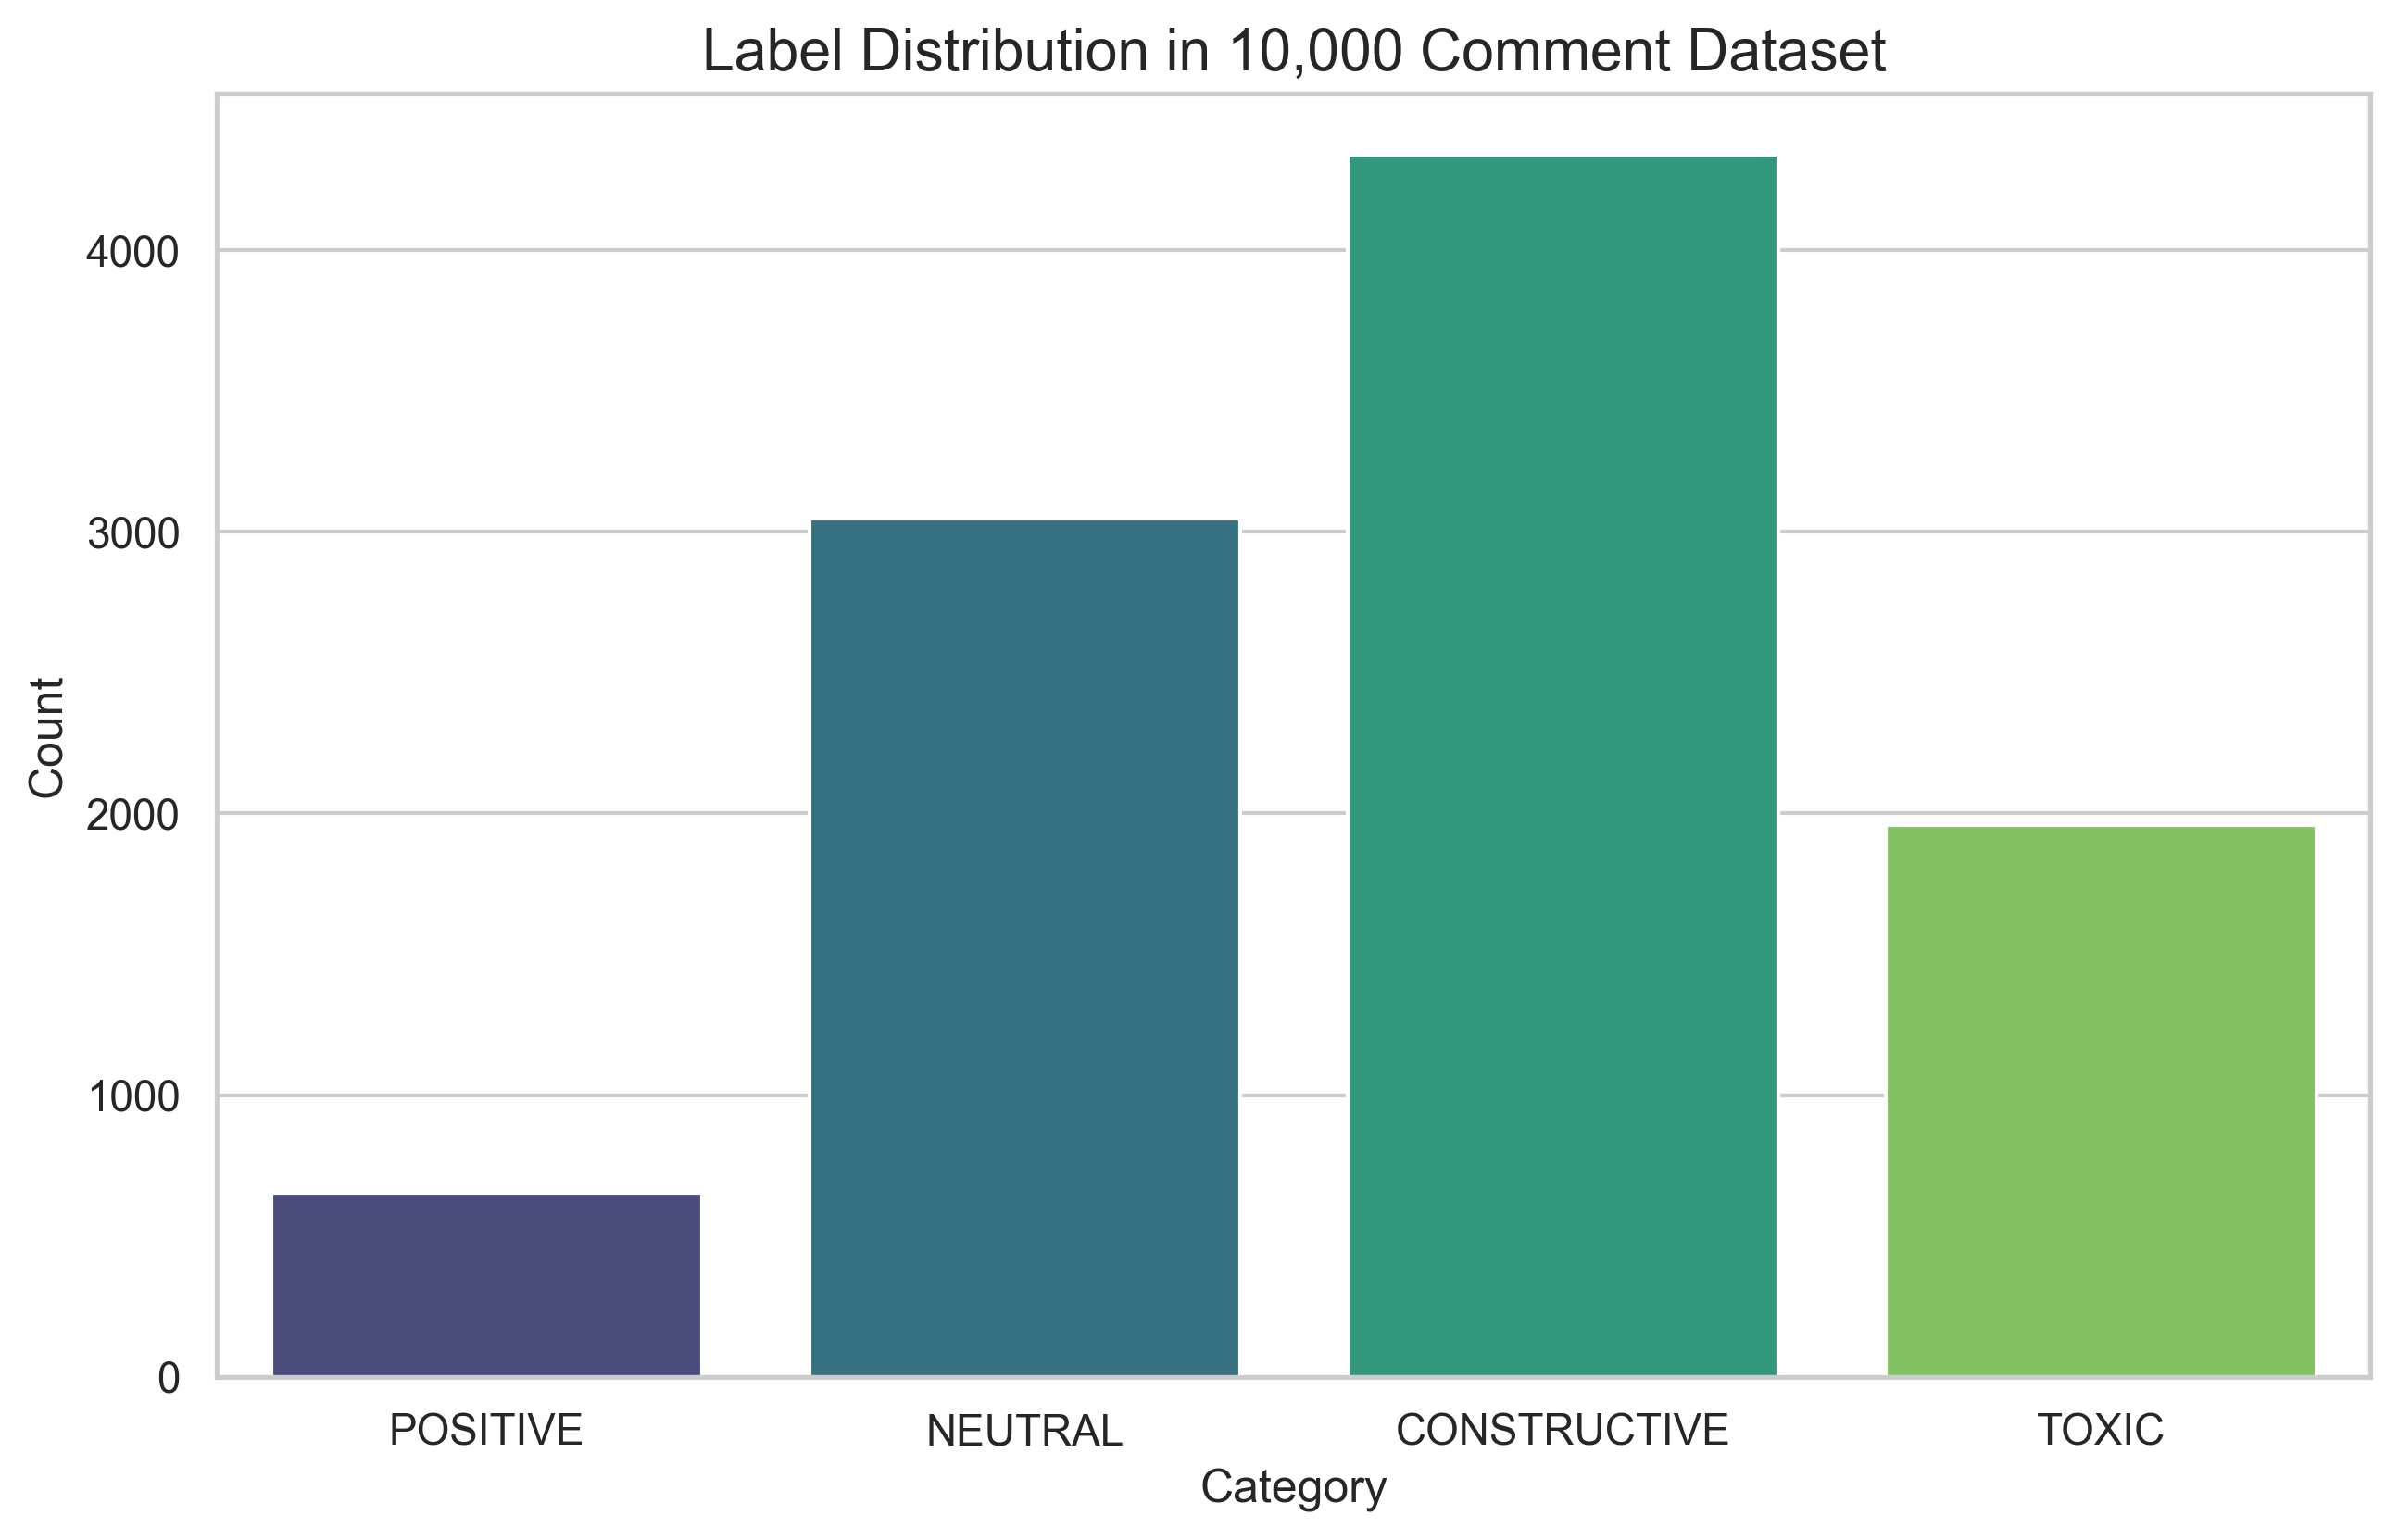
\includegraphics[width=0.8\textwidth]{Figures/EDA/label_distribution.png}
    \caption{10,000 сэтгэгдлийн ангиллын тархалт (зохиогчийн бэлтгэсэн өгөгдөл)}
    \label{fig:label-dist}
\end{figure}

\textbf{Сэтгэгдлийн дундаж урт шинжилгээ.} Сэтгэгдлийн урт гэдэг нь нэг
сэтгэгдэлд орсон нийт тэмдэгтийн тоог хэлнэ. Ангилал тус бүрийн сэтгэгдлийн
медиан уртыг харьцуулан судалсан (Зураг \ref{fig:len-dist}). Бүтээлч шүүмжлэл
ангиллын сэтгэгдлүүд хамгийн урт (median $\approx 137$ тэмдэгт)
байгаа нь --- шүүмжлэгчид өөрийн байр сууриа тайлбарлах, аргумент гаргах,
шийдэл санал болгохдоо илүү урт өгүүлбэр ашиглахтай холбоотой. Харин
Саармаг сэтгэгдлүүд хамгийн богино (median $\approx 59$ тэмдэгт), Хортой сөрөг
($\approx 93$) болон Эерэг ($\approx 90$) нь дунд зэрэг урттай байна --- хортой
агуулга ихэвчлэн богино, шууд халдлага хэлбэрт гарч ирдэгтэй нийцнэ.

\begin{figure}[H]
\centering
\begin{tikzpicture}
\begin{axis}[
  xbar,
  width=10cm, height=5.5cm,
  bar width=0.5cm,
  xlabel={Сэтгэгдлийн медиан урт (тэмдэгт)},
  ytick={1,2,3,4},
  yticklabels={Хортой сөрөг, Саармаг, Эерэг, {Бүтээлч шүүмжлэл}},
  xmin=0, xmax=185,
  nodes near coords,
  nodes near coords align={horizontal},
  every node near coord/.style={font=\small},
  enlarge y limits=0.25,
  tick label style={font=\small},
  label style={font=\small},
]
\addplot[fill=blue!40] coordinates {
  (93,1)
  (59,2)
  (90,3)
  (137,4)
};
\end{axis}
\end{tikzpicture}
\caption{Ангилал тус бүрийн сэтгэгдлийн медиан урт (тэмдэгтийн тоо)}
\label{fig:len-dist}
\end{figure}

\textbf{N-gram давтамжийн шинжилгээ.} Хортой сөрөг болон Бүтээлч шүүмжлэл
ангиллын үгсийн санг ялгахын тулд хамгийн их давтагдсан нэгт үгс (unigrams) болон
хоёртын үгс (bigrams)-ийг шинжлэв. Хортой сөрөг ангилалд хувь хүн рүү чиглэсэн
доромжлол, хараалын үгс давамгайлж байгаа бол, Бүтээлч шүүмжлэл ангилалд ``хэрэгтэй'',
``засах'', ``ажлаа хий'', ``болохгүй байна'' гэх мэт асуудал шийдвэрлэх, үр дүн
шаардсан үг хэллэгүүд түгээмэл байна. Хоёр ангиллын үгсийн санны давхцлыг
зураг~\ref{fig:euler-vocab}-д Euler диаграм хэлбэрээр дүрсэлсэн бөгөөд энэхүү
семантик ялгаа нь хоёр шатлалт ангиллын системийн үндсэн логик болдог.

\begin{figure}[H]
\centering
\begin{tikzpicture}[font=\small]

% Two equal circles: r=2.7cm, centers at (-2.0,0) and (2.0,0)
% center distance=4.0cm → overlap region x∈[-0.7, +0.7]

\draw[fill=red!30, fill opacity=0.55, draw=red!70, line width=1.5pt]
  (-2.0, 0) circle (2.7cm);
\draw[fill=blue!28, fill opacity=0.55, draw=blue!68, line width=1.5pt]
  ( 2.0, 0) circle (2.7cm);

% ── TITLES ───────────────────────────────────────────────────────────────
\node[font=\normalsize\bfseries, text=red!75!black]
  at (-2.0, 3.15) {Хортой сөрөг};
\node[font=\normalsize\bfseries, text=blue!75!black]
  at ( 2.0, 3.15) {Бүтээлч шүүмжлэл};

% ── OVERLAP HEADER (x=0: both dists=2.0<2.7 ✓) ──────────────────────────
\node[font=\footnotesize\bfseries, text=gray!65!black, align=center]
  at (0, 1.30) {Нийтлэг\\үгийн сан};

% ── LEFT-ONLY KEYWORDS (x=-3.0: left dist=1.0..2.0<2.7; right dist>5 ✓) ─
\node[font=\small\itshape, text=red!85!black] at (-3.0,  0.80) {\textit{доромжлол}};
\node[font=\small\itshape, text=red!85!black] at (-3.0,  0.20) {\textit{заналхийлэл}};
\node[font=\small\itshape, text=red!85!black] at (-3.0, -0.40) {\textit{гутаах}};
\node[font=\small\itshape, text=red!85!black] at (-3.0, -1.00) {\textit{тэнэг}};
\node[font=\small\itshape, text=red!85!black] at (-3.0, -1.60) {\textit{дайрах}};

% ── OVERLAP KEYWORDS (x=0: both dists=sqrt(4+y²)<2.7 → |y|<1.87 ✓) ─────
\node[font=\small\itshape, text=gray!75!black] at (0,  0.60) {\textit{сөрөг}};
\node[font=\small\itshape, text=gray!75!black] at (0,  0.00) {\textit{муухай}};
\node[font=\small\itshape, text=gray!75!black] at (0, -0.60) {\textit{болохгүй}};
\node[font=\small\itshape, text=gray!75!black] at (0, -1.20) {\textit{буруу}};

% ── RIGHT-ONLY KEYWORDS (x=3.0: right dist=1.0..2.0<2.7; left dist>5 ✓) ─
\node[font=\small\itshape, text=blue!85!black] at ( 3.0,  0.80) {\textit{засах}};
\node[font=\small\itshape, text=blue!85!black] at ( 3.0,  0.20) {\textit{шийдэл}};
\node[font=\small\itshape, text=blue!85!black] at ( 3.0, -0.40) {\textit{хэрэгтэй}};
\node[font=\small\itshape, text=blue!85!black] at ( 3.0, -1.00) {\textit{ажлаа хий}};
\node[font=\small\itshape, text=blue!85!black] at ( 3.0, -1.60) {\textit{сайжруулах}};

\end{tikzpicture}
\caption{Хортой сөрөг ба Бүтээлч шүүмжлэл ангиллын үгсийн санны давхцал.
  Давхцал нь хоёр ангилалд нийтлэг хэрэглэгддэг үгсийн санг илэрхийлнэ.}
\label{fig:euler-vocab}
\end{figure}

%-------------------------------------------------------------------------------
\section{Өгөгдлийн багцын хуваалт}

Цуглуулсан болон шошгологдсон өгөгдлийн багцыг загварыг сургах, тохируулах, туршихад
ашиглах гурван хэсэгт хуваана: сургалтын (training) $7{,}043$ дээж ($70.43\%$),
параметр тохируулгын (validation) $1{,}428$ дээж ($14.28\%$), туршилтын (test)
$1{,}529$ дээж ($15.29\%$). Хуваалт нь stratified байх ---
өөрөөр хэлбэл дөрвөн ангилал бүрийн харьцаа хэсэг бүрд тэнцүү хуваарилагдана.
Энэ арга нь тэнцвэргүй ангиллын нөхцөлд загварын дутуу суралцалтын
(underfitting) болон хэт суралцалтын (overfitting) эрсдлийг бууруулдаг.
Туршилтын хэсэг нь загварын сургалтын явцад огт ашиглагдалгүй, зөвхөн эцсийн
гүйцэтгэлийн үнэлгээнд нэг удаа ашиглагдана.

\begin{table}[H]
\centering
\caption{Өгөгдлийн багцын ангилал бүрийн жишээний тоо (10,000 дээж)}
\label{tab:data-stats}
\fittable{%
\begin{tabular}{@{}p{4.5cm}cccc@{}}
\toprule
\textbf{Ангилал} & \textbf{Train (70.4\%)} & \textbf{Val (14.3\%)} & \textbf{Test (15.3\%)} & \textbf{Нийт} \\
\midrule
Эерэг     & $475$  & $93$  & $87$  & $655$ \\
Саармаг      & $2{,}109$ & $451$ & $466$ & $3{,}026$ \\
Хортой сөрөг        & $1{,}369$ & $300$ & $294$ & $1{,}963$ \\
Бүтээлч шүүмжлэл & $3{,}090$ & $584$ & $682$ & $4{,}356$ \\
\midrule
\textbf{Нийт} & $\mathbf{7{,}043}$ & $\mathbf{1{,}428}$ & $\mathbf{1{,}529}$ & $\mathbf{10{,}000}$ \\
\bottomrule
\end{tabular}}
\end{table}

\subsection{Өгөгдлийн чанарын үзүүлэлтүүд}

Датасетын чанарыг guideline-ийн шаардлагын дагуу дараах үзүүлэлтээр
баталгаажуулав (Хүснэгт~\ref{tab:data-quality}). Туршилтын хуваалт нь
сургалтын хэсэгтэй давхцалгүй (data leakage $0\%$) бөгөөд давхардсан мөр,
дутуу утга илрээгүй.

\begin{table}[H]
\centering
\caption{Өгөгдлийн чанарын үзүүлэлтүүд}
\label{tab:data-quality}
\begin{tabular}{@{}lcc@{}}
\toprule
\textbf{Үзүүлэлт} & \textbf{Хэмжсэн утга} & \textbf{Зорилтот} \\
\midrule
Ангиллын тэнцвэр (max:min)        & $\approx 6.6{:}1$ (тэнцвэргүй, нөхсөн) & --- \\
Дутуу утгын хувь (missing rate)   & $0.0\%$ & $<5\%$ \\
Давхардсан мөрийн хувь (duplicate)& $0.0\%$ & $0\%$ \\
Annotator нийцэл (Fleiss' $\kappa$)& $0.72$ & $\geq 0.7$ \\
Train/test давхцал (leakage)      & $0.0\%$ ($0$ мөр) & $0\%$ \\
\bottomrule
\end{tabular}
\end{table}

%-------------------------------------------------------------------------------
\section{Монгол хэлний онцгой бэрхшээлүүд}

Монгол хэлний NLP-д нийтлэг тулгардаг хэд хэдэн тусгай бэрхшээл байна.
Нэгдүгээрт, agglutinative бүтэц: нэг үгийн үндэст олон дагавар нэмэгдэж, лексик
хэмжигдэхүүн (vocabulary size) огцом нэмэгдэнэ --- энэ нь BoW, TF-IDF зэрэг
арга зүйн гүйцэтгэлийг бууруулдаг. Хоёрдугаарт, бага хэмжээний нийтэд нээлттэй
corpus: Монгол хэлний NLP-д ашиглах том хэмжээний шошгологдсон өгөгдөл туйлын
хомс байгаа нь загварыг сургах, туршихад хүндрэл учруулдаг. Гуравдугаарт,
ярианы болон бичгийн хэлний ялгаа: нийгмийн сүлжээнд ашиглагдах ярианы хэл нь
стандарт бичгийн Монгол хэлнээс ялгаатай болон тогтворгүй байдаг. Дөрөвдүгээрт,
annotation-ийн нийтлэг стандарт байхгүй: Монгол хэлний хортой агуулгын
шошгологдолтын нийтлэг стандарт, corpus байхгүй тул шошгологчдын хоорондын
нийцлийг хангах нь хүнд байдаг.

\textbf{Кирилл-онцлогт хязгаарлалт.} Энэхүү судалгааны датасет болон загвар нь
зөвхөн кирилл бичгийн Монгол хэлний текстэд хамаарна. Латин үсгийн бичвэр,
монгол-англи холимог (code-switched) текст, латин үсгийн хэлбэртэй Монгол бичлэг (``bn'',
``yu ve'', ``zgr'' гэх мэт хэлбэр), болон кирилл бус бусад бичиглэлийн хэлбэрүүд
одоогийн системийн хамрах хүрээнд ороогүй. Цахим орчинд code-switching нэлээд
тархсан байдаг тул уг хязгаарлалт нь загварын бодит орчин дахь хэрэглээний
хүрээг зарим хэмжээгээр бууруулж болзошгүй. Гэхдээ энэхүү шийдэл нь MN-BERT-ийн
кирилл корпус дээр суурилсан токенчлолын морфологийн тогтвортой байдлыг
хамгаалж, аннотацийн стандартыг нэгтгэхэд шаардлагатай үндэслэлтэй алхам юм.
Латин бичгийн болон code-switched текстийг дэмжих боломжийг ирээдүйн судалгааны
чиглэл болгон тодорхойлно.

%-------------------------------------------------------------------------------
\section{Бүлгийн дүгнэлт}

Өгөгдлийн бэлтгэлийн бүлэгт цуглуулалтын эх сурвалж, цэвэрлэгээний pipeline,
шошгологдолтын стратеги, dataset хуваалт болон Монгол хэлний тусгай бэрхшээлийг
тодорхойлсон. Систем зохион байгуулалтын чанар нь эцэст нь сургалтын өгөгдлийн
чанараас шалтгаалдаг учраас өгөгдлийн бэлтгэлийн энэ бүлэг нь бүхэл ажлын
чухал суурь болдог. Дараагийн бүлэгт системийн архитектур болон загварын зохион
байгуулалтыг нарийвчлан тайлбарлана.
